\chapter{Introduction}\label{chapter:introduction}
In the last few decades, there has been a significant technological development in various fields \cite{techological_evolution}.
Computing technology has advanced rapidly, with the introduction of faster and more powerful processors, and the widespread adoption of cloud computing.\newline
The Internet has also become an integral part of modern life, connecting people and devices across the globe; in addition, the development of faster and more reliable connectivity networks has made it possible to transfer and share data at an even faster rate.\newline
Mobile technology has grown exponentially, thanks to the adoption of smartphones and other mobile devices.\newline
One of the fields that has seen a substantial growth, due to the increasing availability and affordability of devices, sensors and other components, is the Internet of Things (IoT). The term IoT refers to the growing network of physical devices, vehicles, buildings and other items that are embedded with sensors, software and connectivity, which enables these \textit{Things} to collect and share data. These capabilities have the potential to bring significant benefits to society and economy, such as improving public services, increasing efficiency and productivity, and reducing costs.

This technological development is closely connected with the growth of distributed systems. As a consequence of the increase in computing power and the availability of fast and reliable networks, it has become possible to allow devices and systems to work together and share data, even when they are physically separated.

The general growth just discussed brought new challenges, such as the need of engineering complex software which has to take full advantage of the computational infrastructure available, taking in consideration the unpredictability of changes and the heterogeneity of communication required.

In order to face the new complexities it is necessary to rethink and renovate the process of software development.

\textbf{Aggregate Programming} is a paradigm which aims to address these requirements. It allows for the easy manipulation of data across devices, making it possible to perform operation on the data of distributed systems, in a simple and efficient manner.

This paradigm has been implemented in different programming languages and platforms: for example \textbf{Protelis}, \textbf{Scafi} and \textbf{FCPP}. All of them present strengths, but also weaknesses: in order to address those, a new framework can be a solution.

In the following sections of this chapter, these themes are described in details, in order to define the goal of this thesis. Specifically Section \ref{section:aggregate_programming_introduction} describes the aggregate programming characteristics and its main complexities, in Section \ref{section:state_of_the_art} are introduced the implementation of the aggregate paradigm that constitute the current state of the art, and Section \ref{section:motivation_goal} presents the motivations behind this work and the goals that aims to achieve.

\section{Context}\label{section:aggregate_programming_introduction}
In this section it is going to be discussed in details the paradigm of Aggregate Programming, in order to provide the context of its development and an overview about how the paradigm works.

\subsection{Aggregate Programming}
Since the last few decades have witnessed technological advances, the traditional way of engineering software is, in some cases, suboptimal.\newline
The systems developed are becoming more and more complex, with requirements that are sometimes difficult to achieve. 

These challenges are enhanced when coming into terms with distributed systems, because there is the need to handle the always increasing number of connected devices, that share and compute data.\newline
Some relevant complexities are the following \cite{distributed_systems_challenges}:
\begin{itemize}
    \item \textbf{Scalability}: as the number of devices in a distributed system grows, the coordination becomes increasingly complex. This requires the development of scalable algorithms and protocols that can handle large numbers of devices;
    \item \textbf{Heterogeneity and interoperability}: in a distributed system, devices may be made by different manufacturers and use different protocols, which can make it difficult for them to communicate with each other. The interoperability between heterogeneous devices and systems is a major challenge;
    \item \textbf{Synchronization}: devices are usually not connected to a common clock, which can make it difficult to synchronize their activities. This can lead to inconsistencies and errors within the system;
    \item \textbf{Latency}: the distance between devices in a distributed system can lead to high latency, which can affect the performance of the system. Managing and reducing latency is a challenge while coordinating numerous devices;
    \item \textbf{Consistency}: devices may have different views of the system state, which can lead to inconsistencies. Guarantee consistency across devices can be challenging and requires the development of distributed algorithms and protocols;
    \item \textbf{Fault tolerance and error control}: devices may fail or become disconnected, which can disrupt the system. Ensuring fault tolerance and the ability to detect and recover from failures is essential in this kind of systems;
    \item \textbf{Security and privacy}: coordinating devices in a distributed system requires the sharing of sensitive information, which can create security risks.
\end{itemize}

Traditionally, the development of this kind of architectures is focused on the single device, instead of the system as a whole. This means that the developers need to concern about all the aspects just discussed, such as the coordination between devices, creating specific algorithms, but also about security, consistency, fault tolerance, which creates unnecessary complexities during the engineering of a system.\newline
This approach is not feasible when dealing with large-scale, decentralized and adaptive infrastructures, such as the one represented in Figure \ref{fig:iot_connected_things}, which shows an example of a real life environment, with numerous heterogeneous devices that needs to communicate with each others.

\begin{figure}[!ht]
    \centering
    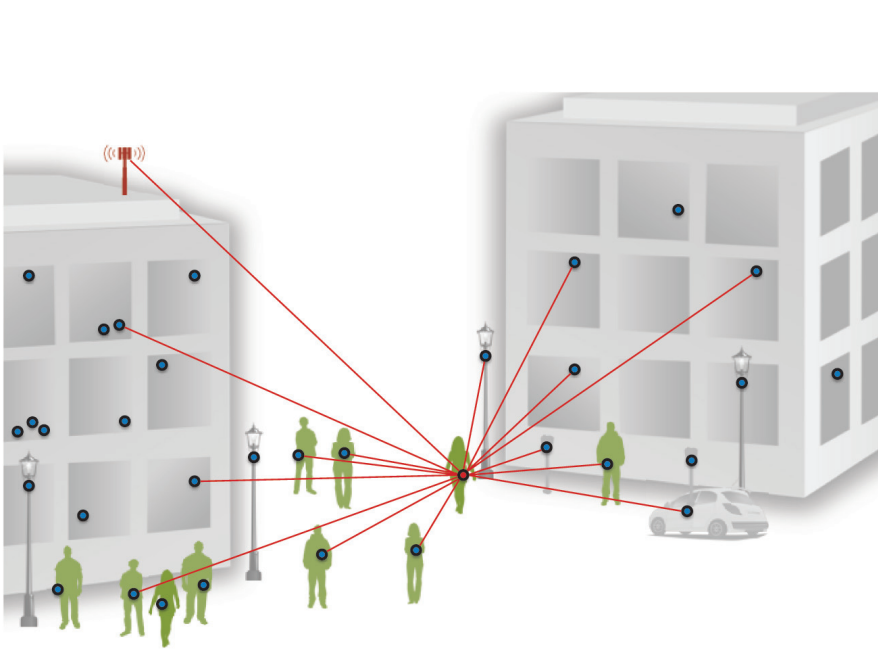
\includegraphics[scale=0.8]{document/chapters/1-introduction/images/iot_connected_things.png}
    \caption{Example of a real life environment, where heterogeneous devices have the possibility to communicate with each other wirelessly creating complex distributed systems. \cite{aggregate_programmig_iot}}
    \label{fig:iot_connected_things}
\end{figure}

Aggregate programming is a paradigm that focuses on the manipulation of complex data structures as a whole, rather than their individual components \cite{aggregate_programmig_iot}. The focus is on what a system is required to do, rather than on how is going to achieve it.\newline
This paradigm is closely related to the \textbf{field calculus} \cite{field_calculus}, a mathematical framework for modeling and reasoning about distributed systems.\newline
Aggregate programming in combination with field calculus, provides a powerful tool for modeling, reasoning, and programming distributed systems. It allows for the efficient manipulation of large and complex data in distributed systems, and facilitates the representation of relationships and interactions between devices. It is a useful approach to adopt for IoT and other distributed systems where scalability, coordination, and security are critical concerns.

The basic concept used in aggregate programming is the \textbf{computational field}, which is a mathematical function that assigns a value to each point in a space, and it is used to represent and manipulate the state of a distributed system.

In order to explain better what a computational field is and how it is used, it is necessary to discuss the assumed computational model \cite{computational_fields_theory}.\newline
Supposing a program P executed by a network of devices defined by a dynamic neighboring relationship. The computation of P can be analyzed by a local and a global point of view.\newline
Considering the \textbf{local} perspective, P is computing on a round-based scheme in single devices. A round is executed in the following steps:
\begin{itemize}
    \item the device sleeps for a delta of time and at some point it wakes up;
    \item it retrieves the information received from neighbors while it was sleeping. The messages sent by the neighbors are fields, and they map the neighbor device identifier with the values computed;
    \item it gathers information about its context;
    \item it retrieves the information stored locally in the previous round about the context;
    \item it executes P, which might manipulate the data of the current context, the data retrieved in the previous round and the neighbors values;
    \item at the end of the execution of P, the device stores the current context's value in the local memory and sent the message to all the neighbors about the current computation;
    \item at the end of the round, the device returns to sleep, until another round begins.
\end{itemize}

On the other hand, the \textbf{global} point of view is the key that makes aggregate computing a powerful tool. In this case, the computation considers the entire network of interconnected devices as a single, unified entity.\newline
The data is represented as a distributed space-time field evolution, which maps the computation events to values computed by devices.\newline
A computational field is a snapshot of the state of the distributed system's network at a certain moment in time, which maps device identifiers to their values.

The main constructs provided by the field calculus are the following:
\begin{itemize}
    \item \textbf{Rep-expression} $rep(e_0)\{(x) \rightarrow e\}$ \newline
    This is the repeat construct, and it represents the time evolution. This allows the field to change dynamically: if in the previous round the rep expression has not been evaluated, the initialization value is $e_0$, otherwise it is the value obtained in the last computation of rep;
    \item \textbf{Nbr-expression} $nbr\{e\}$\newline
    The neighboring is used to model the device-to-neighbor interaction. In order to do this, it is necessary to construct neighboring fields: in this data structure each event is associated to a value, that is mapped to a neighbor identifier and its last value computed. Using this construct it is possible for a device to understand its surrounding by manipulating the neighboring field obtained;
    \item \textbf{Branching} $if(e_0)\{e_1\} else \{e_2\}$\newline
    Branching causes a domain restriction, which means that devices compute $e_1$ only in the restricted domain where $e_0$ is true, otherwise they compute $e_2$. This behavior and its consequences will be discussed in details in Section \ref{subsection:alignment};
    \item \textbf{Function calls} $e(e_1, ..., e_n)$ \newline
    This construct model a function call where $e$ evaluates to a field of function values. 
\end{itemize}

As previously said, the data structures manipulated are distributed over space, and they evolve over time. These two aspects are handled, in the case of field calculus, by two separate constructs: the evolution in time is manipulated by \textit{rep-expression}, the space management, which provide neighbors interactions, is provided by the \textit{nbr-expression}.\newline
The use of time evolution and neighbor interaction operators in the traditional way leads to a slowdown in the efficient spread of information. This is due to the separation of state sharing (nbr) and state updates (rep), which requires information received through nbr to be stored through rep in the local memory of the device before it can be passed on during the next execution of nbr \cite{share_operator}. 

It is possible to overcome this limitation by extending the field calculus with a new construct, which has been called \textbf{share} \cite{share_operator}. The share operator allows to observe the neighbors' field, updated the local values and sharing immediately the updated state in a single computation. It is possible to observe the differences between the behavior of the share operator and the combination of rep and nbr in Figure \ref{fig:share_operator_introduction}.

\begin{figure}[!ht]
    \centering
    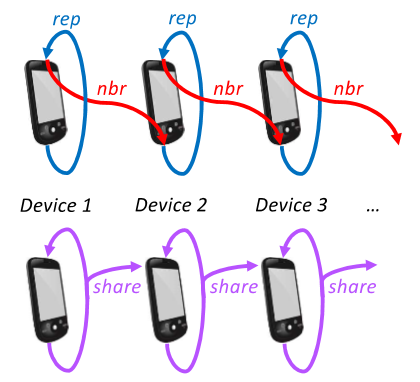
\includegraphics[scale=0.8]{document/chapters/1-introduction/images/share_operator_introduction.png}
    \caption{Comparison between the combination of rep-expression and nbr-expression, and the share construct \cite{share_operator}}
    \label{fig:share_operator_introduction}
\end{figure}

\subsubsection{Domain restriction: alignment}\label{subsection:alignment}
The expected consequence of a branch construct is to determine the portion of code that is going to be computed. In the field calculus, the branch construct also has an unusual behavior, which is called domain restriction.

\begin{lstlisting}
    if (e0) {e1} else {e2}
\end{lstlisting}
Taking in consideration this portion of pseudocode, it is possible to identify two different restricted subdomains: 
\begin{enumerate}
    \item \textbf{$D_{true}$}: this is how the domain is called when $e0$ is true;
    \item \textbf{$D_{false}$}: the name of the domain in the case that the condition $e0$ is false.
\end{enumerate}
For example, if a device is in the domain $D_{true}$, the following are the implications \cite{computational_fields_theory}:
\begin{itemize}
    \item it does not compute $e2$, which is the typical branch behavior;
    \item if $e2$ involves a nbr-expression, this is not going to be evaluated by the considered device. This means that the neighboring devices in $D_{false}$ can not obtain the value of this device for the nbr-expression in $e2$, because it has not been computed. Similarly, the nbr-expression in $e1$ evaluated by this device is not going to be shared from $D_{true}$ to $D_{false}$;
    \item if the device evaluated $e2$ instead of $e1$ in its previous round, then all the rep-expressions in $e2$ are going to be computed using the initialization value.
\end{itemize}

Given this behavior, the result is that devices operating in different subdomains are computing in isolation. As a direct consequence of that they can not communicate with each other unless they are in the same domain. This characteristic is called \textbf{clustering}, which is an important feature: it allows restricting computations in subdomains in an easy and efficient way, which is extremely useful in many use-cases.

The domain restriction is a crucial trait of aggregate programming, and it introduces to a problem that, necessarily, has to be taken in consideration: different devices that operate in a highly distributed system do not possess a shared memory that can be used to keep track of the computation being executed on each device. On the other hand, this domain restriction characteristic requires that each device must communicate only with devices in the same subdomain, which means that they are computing the same operation.

This is defined as the \textbf{alignment problem}, and it is necessary to explore all the information of the system in order to find a solution.

First, it is important to keep in mind that each device has its own identifier, which can be used to define the author of a message.\newline
Second, when dealing with a computational field, such as when retrieving neighboring values using a nbr-expression, the device is currently computing the operation that it is actually looking for in the field.

In order to explain this concept better, here is a snippet of pseudocode:
\begin{lstlisting}
    if (e0) {nbr(e1)} else {nbr(e2)}
\end{lstlisting}
When a device $\delta_1$ is in the domain $D_{true}$, it computes $nbr(e1)$: this means that it is retrieving from the neighbors that computed $e1$, while evaluating $e1$ itself.\newline
Consequently, $\delta_1$ and the other devices have to be aligned in order to exchange information: they are all in the same subdomain, in which $e0$ is evaluated as true, and they are computing $nbr(e1)$.\newline
Given these concepts, it is possible to understand how to deal with the alignment problem: thanks to the current computational location of a device, it is possible to understand which values it is currently trying to retrieve, and, since each device has an identifier, the values can be mapped to those identifiers. Then, combining all the information together, a computational field is obtained.

One thing to notice is that the alignment is not a concern of the branch construct only. In general, the alignment feature is necessary all along an aggregate program, but it can be more clearly noticed in the branch occurrences, which is the reason it has been discussed as the first example.\newline
Considering this pseudocode:
\begin{lstlisting}
fun f1() {nbr(e1)}
fun f2() {nbr(e1)}

f1()
f2()
\end{lstlisting}
Even though the body of the functions $f1$ and $f2$ is the same, they are two different expressions. This means that the neighboring expression in $f1$ is not the same of the one in $f2$, and when one of the neighboring expression is retrieving the values computed by the neighbors, it has to consider only its current computational location. For example if the neighboring expression in $f1$ is executing, it has to get the neighbors' evaluation of the $nbr(e1)$ inside the body of $f1$. The resolution of this problem is the same explained for the branch expression.

Concluding, the alignment is provided by keeping track of the computational location, which must be done every time an aggregate programming expression is involved. In this way it is possible to solve any ambiguity that might appear during the computational field construction.

\section{State of the art}\label{section:state_of_the_art}
The aim of this section is to give an introduction about the state-of-the-art technologies that have been developed in the field of aggregate programming. This overview is going to take in consideration how each implementation works and the choices that led their development, with the goal of depicting a representation of the context in which the project of this thesis is going to be set in.

\subsection{Protelis}\label{subsection:protelis}
Protelis \cite{protelis_introduction} is a functional language inspired by Proto. It implements the field calculus providing a modern specification language.\newline
The architecture is based on Java, and the reasons are multiple:
\begin{itemize}
    \item Java is portable across different systems and devices;
    \item It is easy to import libraries and APIs;
    \item The variety of low-cost embedded devices that are able to support Java is increasing;
    \item Java optimizations in terms of speed and resources consumption are making it a valid alternative to low-level languages, such as C.
\end{itemize}

Since Protelis is a functional language, but its syntax is Java-like, its adoption is not difficult. For example, the following is a snippet of code written in Protelis, which is used to calculate the distance between each device and the source, creating a gradient base on said distance:
\begin{lstlisting}[language=Python, caption=Protelis example, captionpos=b]
def myPosition() = self.getDevicePosition()
def nbrRange() = nbr(myPosition()).distanceTo(myPosition())
share (d <- POSITIVE_INFINITY) {
    let shortestPathViaNeighborhood = 
        foldMin(POSITIVE_INFINITY, d + nbrRange())
    if (env.has("source")) { 
        0 
    } else {
        shortestPathViaNeighborhood
    }
}
\end{lstlisting}

Protelis is very versatile, and it can be used in a wide range of application domains. It is possible to create Protelis modules and execute them in simulations using Alchemist \cite{alchemist}, which is a simulator for pervasive computing and distributed systems.

\subsection{ScaFi}\label{subsection:scafi}
ScaFi \cite{scafi_introduction} is a programming language and framework for Aggregate Programming. Its name stands for \textit{\textbf{Sca}la \textbf{Fi}elds}, since it is built on top of the Scala programming language, which provides the functional programming paradigm and type-safe features. It also uses the Akka framework for actor-based concurrency and the Java Virtual Machine (JVM) for execution.

ScaFi implements a variant of field calculus, providing a domain-specific language (DSL) and API in order to allow writing, testing and running aggregate programs.

One of the key features of ScaFi is its support for declarative programming, which allows developers to specify the desired outcome of a computation, rather than how the computation should be performed. This makes it easier for developers to write correct and efficient distributed algorithms, as they can abstract away the low-level details of communication and synchronization.

ScaFi aims to provide a high-level and type-safe programming interface for building complex systems.\newline
The combination of the Scala programming language, the Akka framework, and the JVM provides a strong foundation for building scalable and robust distributed systems.\newline
In particular, the choice of a JVM-based architecture has the same advantages discussed previously for Protelis (Section \ref{subsection:protelis}), which are mainly portability, low-cost of devices, diffusion and general JVM performances optimizations.

\subsection{FCPP}\label{subsection:fcpp}
FCPP \cite{fcpp_introduction} is a library in C++14, and it implements the field calculus.\newline
It provides tools for simulation of distributed systems, and its extensible component-based architecture makes it suitable for a wide range of application scenarios.

Differently from Protelis and ScaFi, FCPP does not rely on the Java Virtual Machine (JVM). It is implemented in C++, which choice gives the following advantages:
\begin{itemize}
    \item numerous devices support C++ architectures, making it possible deploy FCPP on systems of any sort, which includes microcontrollers;
    \item C++ is performance-oriented, which means that the system requirements are very low, increasing the variety of devices that can use FCCP.
\end{itemize}

These two features allow the coverage of multiple use-cases that were not possible to handle utilizing Protelis and ScaFi: for example the deployment on microcontroller-based systems or cloud applications that have strict parallelism requirements in order to scale correctly, which is guaranteed by the performance improvements.\newline
Since it is based on a lower level language that Protelis and Scafi, programs written in FCCP might be difficult to understand when dealing with complex systems.

\section{Motivation and goal}\label{section:motivation_goal}
When talking about aggregate computing, there are several important features that must be considered when comparing different aggregate programming frameworks, such as ScaFi, Protelis, and FCPP.\newline
After the analysis of the previous sections, it is possible to conclude that:
\begin{itemize}
    \item \textbf{Protelis}\newline
    It has a simple and expressive programming model, but its simplicity and expressiveness come at the cost of performances, as the framework does not provide much control over the underlying data structures and algorithms. Moreover, Protelis might not be the best choice for systems that require strong interoperability with other systems and technologies, since it has a limited set of integrations;
    \item \textbf{ScaFi}\newline
    It has a strong focus on programmability and support for Scala, which can make the system more complex and difficult to understand for developers who are not familiar with the language or the functional programming paradigm. Additionally, ScaFi may have a higher overhead compared to other frameworks due to its use of a more expressive programming model;
    \item \textbf{FCPP}\newline
    The key aspects taken in consideration from FCPP are scalability and performance, providing efficient algorithms and data structures for large-scale data processing. These features can make the framework more complex and difficult to understand, since it utilize a low-level programming model that requires a deep understanding of algorithms and data structures.
\end{itemize}

These considerations highlight crucial weaknesses of the already existent frameworks that the project of this thesis tries to overcome. Specifically, the project is an aggregate programming Domain-Specific Language (DSL) in Kotlin and the main features to achieve are the following:
\begin{itemize}
    \item \textbf{Transparency}: refers to the ability of the DSL to provide clear and concise information about the underlying system's behavior, such as how data is processed, stored, and communicated between nodes in a distributed system. Transparency helps to reduce the complexity of the system and makes it easier to understand and maintain, especially in the case of large and complex systems;
    \item \textbf{Minimality}: refers to the design of the DSL to have as few constructs and abstractions as possible while still providing all the necessary functionality. This makes the system easier to understand, maintain, and debug. Minimality also helps to lower the overhead associated with the use of the DSL, which is especially important for systems that require high performance and scalability;
    \item \textbf{Portability}: refers to the ability of the DSL to run on different platforms and environments, such as different operating systems, cloud platforms, and hardware architectures. Portability helps to ensure that the systems built using the DSL can be easily deployed and run in different environments, which is especially important for systems that need to be deployed in multiple locations or need to scale to meet changing demands.
\end{itemize}

The goal of this thesis is the study and the implementation of the aggregate programming paradigm, facing the alignment problem discussed in Section \ref{subsection:alignment}, focussing on transparency, minimality and portability.\newline
The reminder of this thesis is organized as follows. Chapter \ref{chapter:metaprogramming} debates all the possibilities of metaprogramming in Kotlin, and Chapter \ref{chapter:alignment} explains in details the solution of the alignment problem. Chapter \ref{chapter:collektive} describes how the DSL is implemented and shows the end usage result. Finally, Chapter \ref{chapter:conclusion} summarizes the work done in this thesis, adding plans for future development.
